%%%%%%%%%%%%%%%%%%%%%%%%%%%%%%%%%%%%%%%%%%%%%%%%%%%%%%%%%%%%%%%%%%%%%%%%%%%%%%%
% PART II PROJECT DISSERTATION - RECOMMENDER SYSTEMS
%
% Amir H. Hajizamani, ahh29@cam.ac.uk
%
%%%%%%%%%%%%%%%%%%%%%%%%%%%%%%%%%%%%%%%%%%%%%%%%%%%%%%%%%%%%%%%%%%%%%%%%%%%%%%%

\documentclass[a4paper,12pt,twoside,notitlepage]{report}

\author{Amir H. Hajizamani}
\title{CST Part II Individual Project Dissertation - Recommender Systems for 
Social Networks}

\usepackage{verbatim}
\usepackage[T1]{fontenc}
\usepackage{a4wide}
\usepackage{parskip}
\usepackage{hyperref}
\usepackage{url}
\usepackage{amsmath}
%\usepackage{proof}
\usepackage{comment}

% Conditionals (for draft mode)
\usepackage{ifthen}

% Headers
\usepackage{fancyhdr}

% TOC customisation
\usepackage{tocloft}

% Captions
\usepackage{subfig}
\usepackage{caption}

% Figures
\usepackage{wrapfig}
\usepackage{graphicx}
\usepackage{tikz}
\usetikzlibrary{positioning,mindmap,chains,shapes.misc,arrows,fit}
\usetikzlibrary{decorations.pathmorphing}

% Tables
\usepackage{array}
\usepackage{booktabs}
\usepackage{colortbl}
\usepackage{longtable}

% Palatino font - remove to go back to normal CMR
\usepackage{mathpazo}

% Colour
\usepackage{color}

% Listings (for code snippets ..._
\usepackage{listings}

% Algorithms
\usepackage[boxed]{algorithm}

%\makeindex

\frenchspacing

%%%%%%%%%%%%%%%%%%%%%%%%%%%%%%%%%%%%%%%%%%%%%%%%%%%%%%%%%%%%%%%%%%%%%%%%%%%%%%%
% The BIG DRAFT SWITCH - Set to true to enable draft mode
%
% !!! This will produce extra output that 
%     is not part of the final dissertation !!!

\newboolean{draft}
\setboolean{draft}{true}

%%%%%%%%%%%%%%%%%%%%%%%%%%%%%%%%%%%%%%%%%%%%%%%%%%%%%%%%%%%%%%%%%%%%%%%%%%%%%%%

%%%%%%%%%%%%%%%%%%%%%%%%%%%%%%%%%%%%%%%%%%%%%%%%%%%%%%%%%%%%%%%%%%%%%%%%%%%%%%%
% Definitions

\def\projtitle{Recommender Systems for Social Networks}
\def\authorname{Amir~H.~Hajizamani} 
\def\authoremail{\url{ahh29@cam.ac.uk}}
\def\authorcollege{St.~John's~College}
\def\projsupervisor{Cecilia~Mascolo}

\def\mixurl{\emph{mixcloud.com}}


%%%%%%%%%%%%%%%%%%%%%%%%%%%%%%%%%%%%%%%%%%%%%%%%%%%%%%%%%%%%%%%%%%%%%%%%%%%%%%%
% Custom Environments

\newcommand{\fixme}[1]{\ifdraft{\color{red} {\bf Fixme: \sc #1}}\fi}
\newcommand{\todo}[1]{\ifdraft{\textsf{\color{red} TODO: #1}}\fi}
\newcommand{\remark}[1]{\ifdraft{\textsf{\color{blue} #1}}\fi}

% Some formatting shortcuts
\newcommand{\rulewidth}{300pt}
\newcommand{\halfrule}{
  \begin{center}
    {\rule{\rulewidth}{0.5pt}}
  \end{center}}

%% Colours
\definecolor{darkgreen}{rgb}{0,0.3137,0.196}
\definecolor{commentgreen}{rgb}{0.247,0.5,0.3725}
\definecolor{darkpurple}{rgb}{0.5,0,0.33}

%% Some shortcuts for maths stuff
\providecommand{\Fm}{\mathtt{F}}
\providecommand{\Pm}{\mathtt{P}}
\providecommand{\Tp}{\textsuperscript{\textsf{T}}}
\providecommand{\xsub}[1]{\mathbf{x}_{#1}}
\providecommand{\X}{\mathbf{X}}
\providecommand{\Pmc}[2]{\mathbf{p}_{#1}^{#2\textsf{T}}}

%% TikZ command for line annotations
% Draw line annotation
% Input:
%   #1 Line offset (optional)
%   #2 Line angle
%   #3 Line length
%   #4 Line label
%   #5 Line colour
% Example:
%   \lineann[1]{30}{2}{$L_1$}
\newcommand{\lineann}[5][0.5]{%
    \begin{scope}[rotate=#2, #5,inner sep=2pt]
        \draw[dashed, #5!40] (0,0) -- +(0,#1)
            node [coordinate, near end] (a) {};
        \draw[dashed, #5!40] (#3,0) -- +(0,#1)
            node [coordinate, near end] (b) {};
        \draw[|<->|] (a) -- node[fill=white] {#4} (b);
    \end{scope}
}

%%%%%%%%%%%%%%%%%%%%%%%%%%%%%%%%%%%%%%%%%%%%%%%%%%%%%%%%%%%%%%%%%%%%%%%%%%%%%%%

\setcounter{page}{1}    % initialise page counter

% pre-TOC page formatting
\pagenumbering{roman}
\pagestyle{plain}

\setcounter{secnumdepth}{2}
\setcounter{tocdepth}{3}

\setlength{\parindent}{0pt}
\setlength{\parskip}{6pt}
\linespread{1.2}

\lstset{    basicstyle=\footnotesize\ttfamily, 
            keywordstyle=\color{purple},
            commentstyle=\color{commentgreen}\textit,
            captionpos=b
        }

\begin{document}

%%%%%%%%%%%%%%%%%%%%%%%%%%%%%%%%%%%%%%%%%%%%%%%%%%%%%%%%%%%%%%%%%%%%%%%%%%%%%%%
% Title Page

\thispagestyle{empty} 

\begin{flushright}
\authorname
\end{flushright}
\bigskip % have this so that vfill works to centre the title vertically

\vfill

\begin{center}
 \medskip
 {\Large\bf \projtitle}

 \vspace*{1cm}

 {\large Computer Science Tripos Part II}

 \bigskip

 {\large \authorcollege}

 \bigskip

 {\large \today}
\end{center}

\vfill

\cleardoublepage


%%%%%%%%%%%%%%%%%%%%%%%%%%%%%%%%%%%%%%%%%%%%%%%%%%%%%%%%%%%%%%%%%%%%%%%%%%%%%%%
% Proforma
\section*{Proforma}

\begin{tabular}{ll}
Name:               & \bf \authorname \\
College:            & \bf \authorcollege \\
Project Title:      & \bf \projtitle \\
Examination:        & \bf Computer Science Tripos, Part II, June 2011 \\
Word Count:         & \bf \todo{~4000 words atm} \\
Project Originator: & \bf \authorname \\
Supervisor:         & \bf \projsupervisor \\
\end{tabular}

%\footnotetext[1]{This word count was computed
%by {\tt detex diss.tex | tr -cd '0-9A-Za-z $\tt\backslash$n' | wc -w}}

\subsection*{Original Aims of the Project}

To build a system that would recommend new social links to users of a social
network in order to increase the connectivity of its social graph. These
recommendations would be based on the current state of the graph and their
quality would depend on whether the recommended links actually occur in a
future state of the graph. From the outset, the dataset to be used for the
project was that of the online audio-sharing community \mixurl.

\subsection*{Work Completed}
I modelled the Mixcloud dataset's entities and wrote an abstraction layer for
the Mixcloud API. I used this in a crawler program that downloaded and stored
the data on \mixurl.

The recommender system I wrote achieves the above aims by modelling the
recommendation process as an edge prediction problem: given a social graph,
it tries to predict what edges are most likely to form in the future between
unconnected nodes and assigns a confidence value to the predictions. This is
done by calculating similarity values between nodes and choosing the most
similar unconnected nodes as predictions.

\subsection*{Special Difficulties}

None.

\newpage

%%%%%%%%%%%%%%%%%%%%%%%%%%%%%%%%%%%%%%%%%%%%%%%%%%%%%%%%%%%%%%%%%%%%%%%%%%%%%%%
% Declaration of Originality
\section*{Declaration}

I, \authorname~of \authorcollege, being a candidate for Part II of the Computer
Science Tripos, hereby declare that this dissertation and the work described in
it are my own work, unaided except as may be specified below, and that
the dissertation does not contain material that has already been used to any
substantial extent for a comparable purpose.

\bigskip
\bigskip
\bigskip
\leftline{Signed}

\medskip
\leftline{Date}


\clearpage

%%%%%%%%%%%%%%%%%%%%%%%%%%%%%%%%%%%%%%%%%%%%%%%%%%%%%%%%%%%%%%%%%%%%%%%%%%%%%%%
% Acknowledgements

\section*{Acknowledgements}

If this dissertation turns out to be anything worth the paper it's printed on I
have the following people to thank:

\begin{itemize}
 \item {\bf Liam~McNamara}, for all the insightful advice along the way and
generally being an awesome guy.
 \item {\bf Helen~Ennos}, for all her encouragement and support. Without her, my
time at Cambridge would have been a very different experience. 
\end{itemize}

\cleardoublepage

%%%%%%%%%%%%%%%%%%%%%%%%%%%%%%%%%%%%%%%%%%%%%%%%%%%%%%%%%%%%%%%%%%%%%%%%%%%%%%%
% Table of Contents
\tableofcontents
\clearpage

\clearpage
\listoffigures

\clearpage
\listoftables

\clearpage
\lstlistoflistings

\cleardoublepage


%%%%%%%%%%%%%%%%%%%%%%%%%%%%%%%%%%%%%%%%%%%%%%%%%%%%%%%%%%%%%%%%%%%%%%%%%%%%%%%

% Switch to arabic page numbers after TOC
\setcounter{page}{1}
\setcounter{chapter}{0}
\pagenumbering{arabic}
\pagestyle{headings}


%%%%%%%%%%%%%%%%%%%%%%%%%%%%%%%%%%%%%%%%%%%%%%%%%%%%%%%%%%%%%%%%%%%%%%%%%%%%%%%
% Introduction
\chapter{Introduction}

% - Mention fulfillment early
% - Principal Motivation
% - Other CS work

In this chapter I will explain my motivations for investigating recommender
systems in general and the specific focus points of my project as
presented in this dissertation using data from \mixurl.

\halfrule

\section{Motivation}

The basic concept that underpins recommender systems is that the value of data
about an individual person or piece of content is increased by knowledge of its
relation to other such entities. This is true for the user of a system, whose
experience is enriched with this metadata and is thus incentivised to keep
using, it and the service provider, whose cultural impact and financial success
will depend the growth and interactions of its users with the service.

There are now a growing number of available social networking services that
individuals can choose to invest time and effort into. We take this investment
by the user to consist of: providing personal information, creating and sharing
content, making social connections with other users, and interacting with other
users and content. One way of providing an incentive to do this is by making it
easier for users to make \emph{discoveries} -- to find other individuals or
items of interest (real-world friends, content that compliments the user's
favourites). That is, make recommendations to users and keep them interested in
exploring what the social network has to offer. Recommender systems aim
to solve the problem of \emph{information overload} in areas where the users of
a service struggle to make good choices on what content to consume or what
social activities to take part in, simply because the options are overwhelming.

If we treat the users of a social network as a community, it is clear that such
a community will need the investment mentioned above from its users to reach
some critical mass -- the point at which it is valuable for others to join 
or contribute to the network\footnote{Best described by Beckstrom's Law - The
value of a network equals the net value added to each user's transactions
conducted through that network, summed over all users.} because the majority of
their friends have, or so much of the content they consume is accessible via the
service. This will continually increase the richness and quality of the service
the community receives (assuming the service provider keeps up and adapts to
changes!) and increase the lifetime and utility of the service for its users,
too. Of course, here we are concerned with social networks that aim to reach the
mainstream and are not inherently limited to a select number of users. For
instance, a social network for the community of world experts on network
congestion analysis is bound to hit its maximum membership limit very quickly
and not be much more useful to its users than email or more traditional
communication methods.

From a commercial perspective of a service provider, having users remain active
on the network and incentivise others to do so, too, is paramount. It is
well-understood that social network service providers are not expected to be
profitable\footnote{The 
risks underlying the business of social networks -- 
\url{http://www.makeuseof.com/tag/how-do-social-networks-make-money-case-wondering/}} 
until they reach an ``audience of scale'' to enable the adoption of a sensible 
monetisation model. For instance, Facebook only became profitable in 2009\footnote{
\url{http://www.pcpro.co.uk/news/351646/facebook-eyes-profit-as-it-hits-300-million-members}} 
after reaching 300 million users. This means that the investors who enable such 
ventures at the start need to be convinced that the service has the potential 
to reach popularity and therefore provide a return on investment. Of the many 
strategies that can be used to maintain the growth of a social network, 
implementing a good friend recommender system is standard practice. It should be
noted that recommendations are difficult, if not infeasible, to make at the
very beginning of a network's lifetime due to the \emph{cold start} problem,
that is, when there is insufficient data to base recommendations on. Therefore,
the focus of this project is on stages of a network's lifetime when it is
nearing maturity and this issue hasbeen overcome.

\subsection{Wider Context}

The Web is rife with successful recommender systems, with companies such as 
\emph{Amazon, Netflix\footnote{In 2006 Netflix challenged programmers to 
improve their movie recommendation engine by 10\%.}} and \emph{Pandora} 
(radio service backed by \emph{The Music Genome Project}\footnote{The MGP 
uses the``genealogy'' of music to link songs and artists -- 
\url{http://www.pandora.com}}) investing a lot of time and money in improving 
their algorithms and data quality to better recommend items of interest to 
their users. On the other hand, more directly community-driven websites such as 
\emph{del.icio.us} and \emph{flickr} have harnessed the collective 
intelligence of their users and their tagging of their content with keywords. 
Collaborative tagging leads to an organic categorisation and annotation of data 
which has been termed \emph{folksonomy}\footnote{A portmanteau of 
\emph{folk} and \emph{taxonomy} -- 
\url{http://www.vanderwal.net/folksonomy.html}}. In a sufficiently large and 
active community, the folksonomy that can be extracted becomes a good source of 
input for the algorithms in a recommender system. 

With the accelerating growth of social networks such as Twitter and Facebook, 
the value of social recommendations which aim to increase the connections 
between individuals is more important that it used to be: the items of 
interests are now other users not products on sale (though from an advertising 
revenue perspective the difference is blurred). Recommender systems are nearing 
maturity and will soon be, if they are not already, commodity technologies as 
the ``social connections layer'' of virtual communities is completed\footnote{
The ``game layer'' is the next stage in building virtual communities, the 
founder of SCVNGR argues -- \url{
http://www.ted.com/talks/seth_priebatsch_the_game_layer_on_top_of_the_world.html
}}. 
This means that an analysis of such systems is essential to the understanding 
of social networking and the Web as it experiences a paradigm shift from a 
\emph{search} platform (e.g. Google) to a \emph{discovery} platform.


\section{The \mixurl\ Dataset}

\mixurl\ are a successful audio content distribution website, aiming to be the
``YouTube of Radio''. They provide a platform for user-generated audio content,
ranging from podcasts to DJ mixes, to be easily accessed by anyone. They have
been operating for nearly two years and have in the order of 100,000 users and a
similar number of so-called ``Cloudcasts'' (uploaded audio content). They
provide their niche community of users with social networking features such as
Twitter-style following, Facebook-style activity updates, favouriting of
Cloudcasts and commenting, and a record of listening history. The user-uploaded
Cloudcasts are also heavily annotated with tags, categories, text descriptions
and other metadata. This wealth of metadata about Mixcloud's users and content
is available via their public API\footnote{\url{http://api.mixcloud.com}} and I
gathered the data I need from it.

\subsection{Focus on Social Recommendations}
At the time of writing, \mixurl\ implements some simple mechanisms for 
\emph{item recommendations} and \emph{personalised recommendations}: 
respectively, recommending Cloudcasts similar to the one being viewed/played,
and recommending Cloudcasts related to the user's personal listening history. 

My approach is to provide \emph{social recommendations}: suggesting \emph{other
users} whom the current user may be interested in following or listening to. My
reason for this is that the social aspect of the \mixurl\ community is more
similar to that of Twitter, where people connect with users who produce good
content as well as real life friends, than that of Facebook where social links
are more often initiated physically, or in the traditional sense of ``social''.

Given the motivations for building recommender systems described above, I
understand that the Mixcloud team have prioritised the implementation of 
the recommendations centred around content because their main
focus has been on building up the library of content on their network and
promoting themselves as content distributors. However, the social networking
layer on top of their distribution layer is the next natural focus. 

\subsection{The Temporal Dimension}

As I am collecting my own data firsthand, I can look at the performance of my
recommendations over temporal snapshots of the dataset. This approach could be
very interesting because changes to the dataset over time provide the ground
truths that my recommender system would be trying to replicate, since I am
approaching recommendations as the same as making predictions.

\todo{more detail here?}

\subsection{Comparison with other Available Datasets}

The most widely used datasets in discussions on recommender systems are the 
MovieLens, EachMovie, Book-Crossing and Jester Jokes datasets\footnote{
All of these datasets are available via\url{http://www.grouplens.org/node/12}} 
which contain items and user ratings on their respective titular item types. 
Though the quality of these datasets is proven, they have limitations for my 
intended project goals. In particular, there is no social connectivity data 
between users in these datasets and the links between entities are limited to 
ratings by users on some items. With the Mixcloud dataset I am able to explore 
the social graph of the users. Furthermore, the Mixcloud dataset provides much 
richer metadata about its entities, as described above, than any of these 
traditional datasets which give only enough data to make item
recommendations. The Mixcloud dataset has scope for more interesting analysis.

%%%%%%%%%%%%%%%%%%%%%%%%%%%%%%%%%%%%%%%%%%%%%%%%%%%%%%%%%%%%%%%%%%%%%%%%%%%%%%%
% Preparation 
\chapter{Preparation}

This chapter describes how I refined the ideas presented in my project proposal
before writing any code, and the working environments and best practices I
adopted to minimise problems during the implementation stage.

\halfrule

\section{The Anatomy of the \mixurl\ Dataset}
\label{sec:mix-anatomy}

It is important to understand the nature of the dataset that I use in this
project. What follows is some semantics of how the data is structured, accessed
and presented. 

The general notion underlying \mixurl\ is that producers of audio
content (so-called \emph{Cloudcasts}) and their listeners are users of the
website, and any user can upload content with rich metadata including artist and
track information. The users can then listen to and favorite content, and
furthermore, they can follow other users in whom they are interested, either
socially or because of their content.

All the above data can be obtained from Mixcloud via their Application
Programming Interfact (API) and I break this down in the following subsections.

\begin{figure}
 \centering
 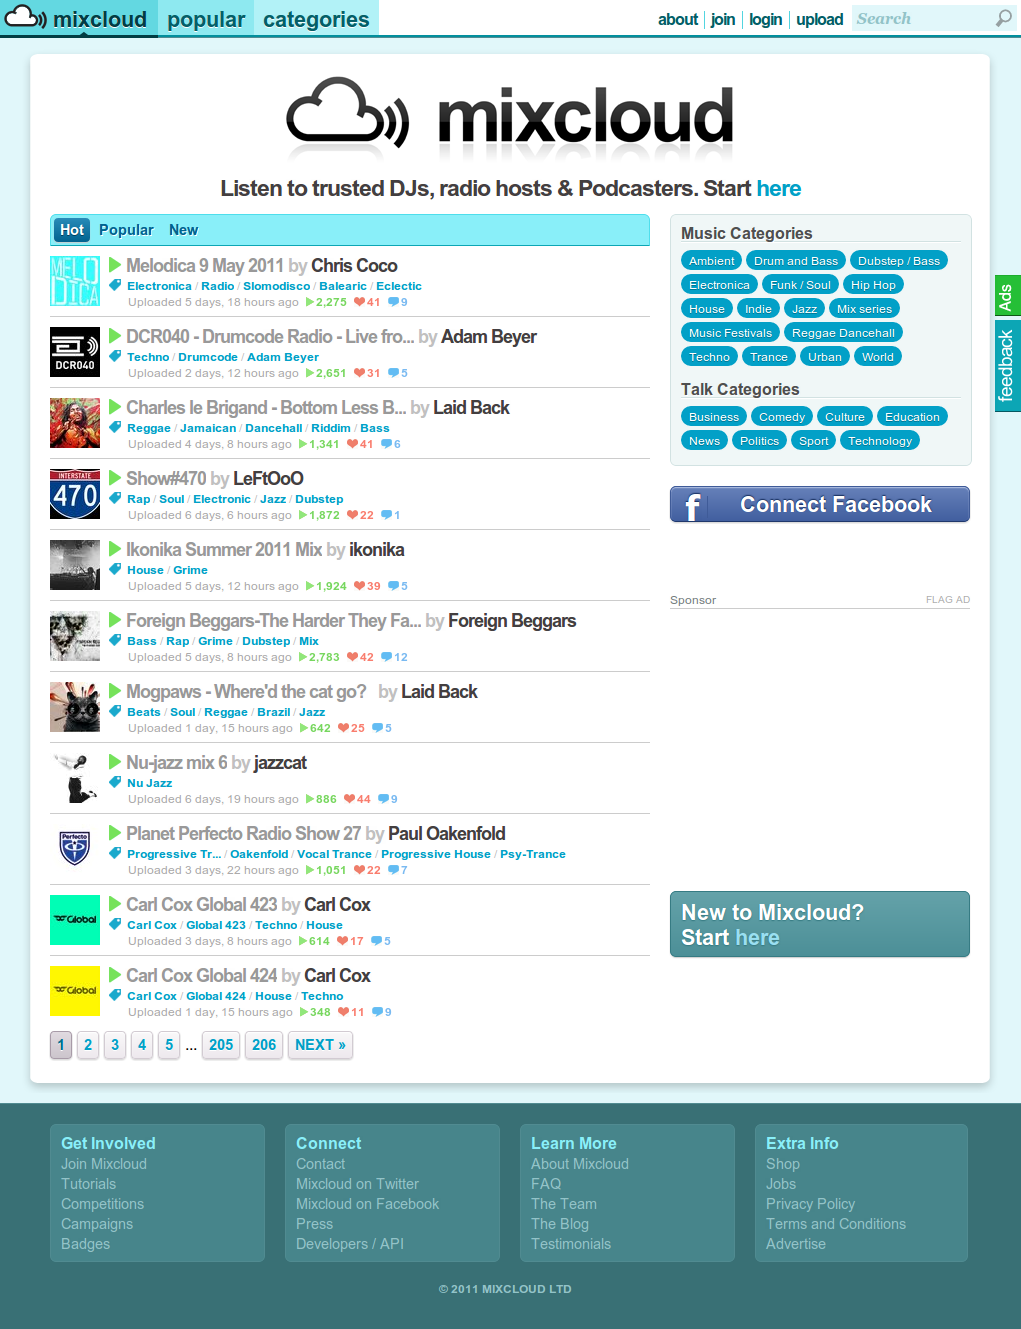
\includegraphics[width=\textwidth]{./images/mixcloud-home.png}
 % mixcloud-home.png: 1021x1329 pixel, 72dpi, 36.02x46.88 cm, bb=0 0 1021 1329
 \caption{\mixurl\ Homepage}
 \label{fig:mix-home}
\end{figure}

\begin{figure}
 \centering
 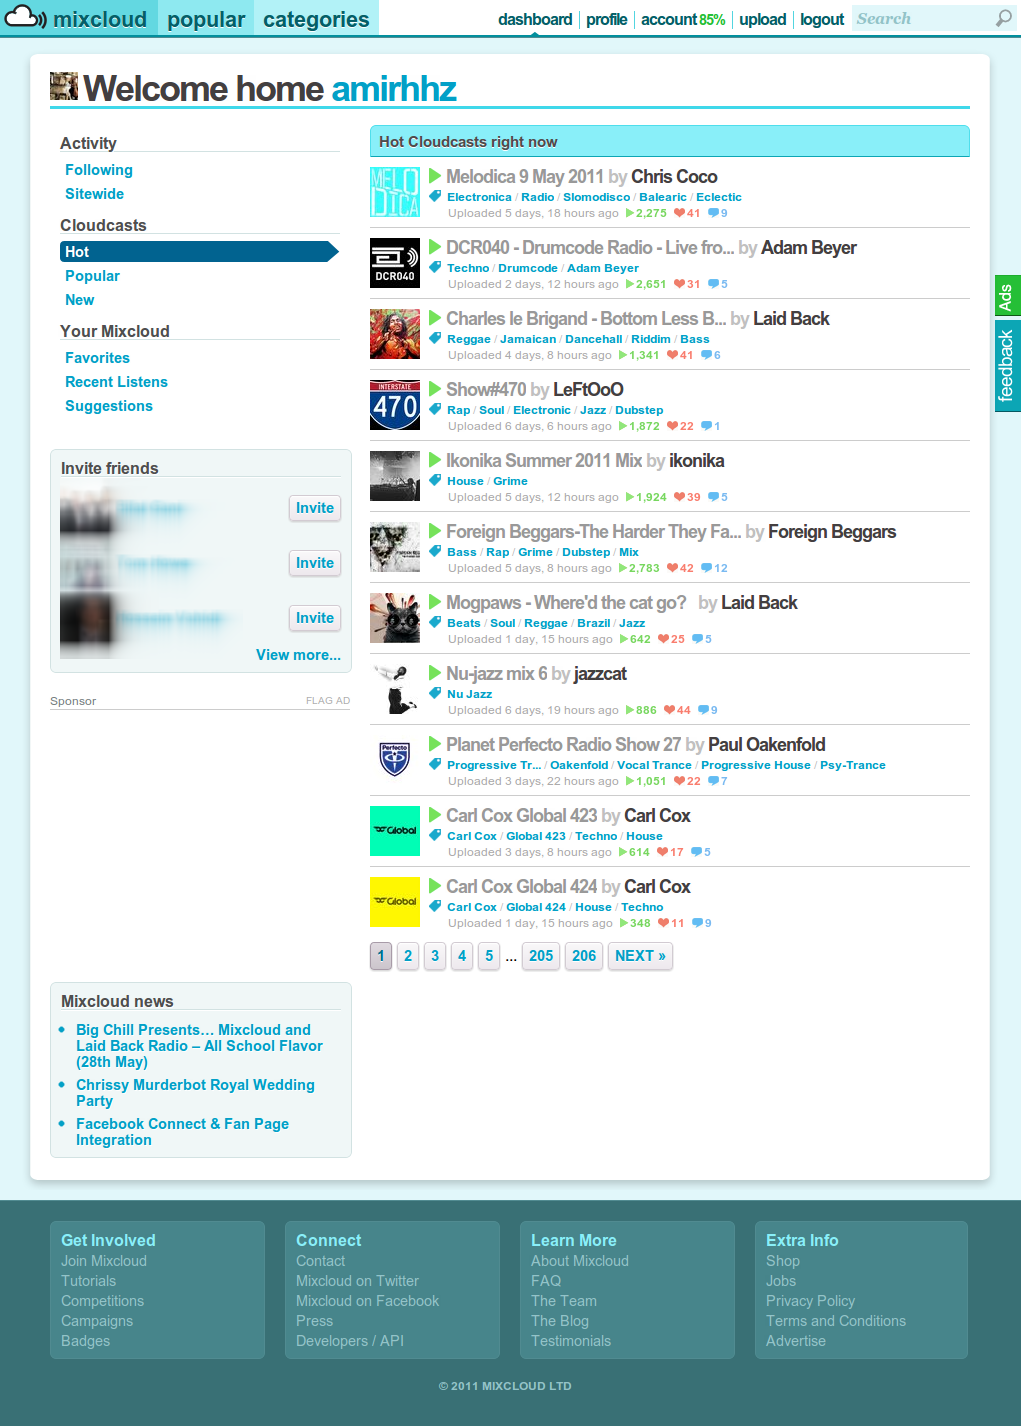
\includegraphics[width=\textwidth]{./images/mixcloud-dashb.png}
 % mixcloud-home.png: 1021x1329 pixel, 72dpi, 36.02x46.88 cm, bb=0 0 1021 1329
 \caption{\mixurl\ Dashboard for logged-in user}
 \label{fig:mix-dash}
\end{figure}

\subsection{The Mixcloud API: A RESTful Exchange of JSON}

The Mixcloud API, accessible via HTTP requests on \url{http://api.mixcloud.com},
allows for the retrieval of data about the various entities and relationship
described above, such as users and cloudcasts. The API responds to HTTP methods
with a JSON\footnote{JavaScript Object Notation}-formatted representation of
the data (see subsection \ref{subsec:nonrel} for more details) for the resource
specified by the URL path. So, for instance, a HTTP
GET request sent to \url{http://api.mixcloud.com/amirhhz} will respond with a
body containing my user information as follows:

\begin{lstlisting}[language=Java,caption=Sample response from the Mixcloud API,
label=lst:api-sample]
{
    "username": "amirhhz", 
    "city": "", 
    "cloudcast_count": 0, 
    "following_count": 11, 
    "url": "http://www.mixcloud.com/amirhhz/", 
    "pictures": {
        "small": /* URL OMMITTED */, 
        "large": /* URL OMMITTED */, 
        "medium": /* URL OMMITTED */, 
    }, 
    "listen_count": 20, 
    "updated_time": "2011-04-13T18:36:57Z", 
    "created_time": "2009-09-07T19:10:17Z", 
    "biog": "", 
    "key": "/amirhhz/", 
    "country": "United Kingdom", 
    "follower_count": 28, 
    "favorite_count": 4, 
    "name": "amirhhz"
} 
\end{lstlisting}

The Mixcloud API adheres to the Representational State Transfer (REST)
style of software architecture, a simple idiom: clients send requests for the
state of a resource to servers and receive an appropriate response containing a
representation of the resource's state at the time. HTTP follows this simple
idiom with its simple methods (e.g. GET, POST, DELETE) and RESTful API's such as
Mixcloud's simply specialise this mechanism to suit their needs of Creating,
Reading, Updating, and Deleting (CRUD) resources on servers as requested by
clients.

\subsection{Base Resources}
In the context of the Mixcloud API, I shall refer to resources in Table 
\ref{tab:base-resources} as \emph{base
resources}.


\begin{table}[h]
  \begin{center}
  \begin{tabular}{r >{\ttfamily}l<{\normalfont}}
Base Resource 	& \textnormal{API path scheme} \\
\hline
User 		& /<user>/ \\
Cloudcast	& /<user>/<cloudcast>/ \\
Tag 		& /tag/<tag>/ \\
Category 	& /categories>/<category>/ \\
Artist 		& /artist/<artist>/ \\
Track		& /track/<artist>/<trackname>/ \\

  \end{tabular}
   
  \end{center}
\caption{Mixcloud API Base Resources and their path schemes}
\label{tab:base-resources}
\end{table}

The main characteristic of base resources is that once they are created the
content of their API data changes rarely or by minimal amounts, as opposed to
the dynamic resources listed below in Table \ref{tab:dyn-resources}.

%\todo{Adding the "metadata=1" argument includes links to their dynamic
%resources, too, as listed further down e.g.
%"http://api.mixcloud.com/amirhhz/?metadata=1".}


\subsection{Dynamic Resources}
Each base resource has some \emph{dynamic resources} associated with
it which effectively return the results of queries on the base resources, for
example, ``who are the followers of user X?''. These are shown in Table
\ref{tab:dyn-resources}.

\begin{table}[h]
  \begin{center}
  \begin{tabular}{r >{\ttfamily}l<{\normalfont}}
Dynamic Resource 	& \textnormal{Path to add to to base resource} \\
\hline
Activity feed 	& feed/ \\
List of followers & followers/ \\
List of followees & following/ \\
Associated comments & comments/ \\
Favorited cloudcasts & favorites/ \\
Uploaded cloudcasts & cloudcasts/ \\
Cloudcasts listened to & listens/ \\
Listeners of a cloudcast & listeners/ \\
Similar cloudcasts & similar/ \\
Popular cloudcasts & popular/ \\
New cloudcasts & new/ \\
Associated users & users/ \\
Staff-picked associated users & userpick\_users/ \\
Staff-picked associated cloudcasts & userpick\_cloudcasts/ \\
  \end{tabular}
   
  \end{center}
\caption{Mixcloud API Dynamic Resources}
\label{tab:dyn-resources}
\end{table}

The required response from these dynamic resource may span several
so-called ``pages`` of JSON data which are navigated by by adding HTTP
arguments to the dynamic resource URL (e.g. \texttt{?offset=0\&limit=100}).

%And there are these miscellany of resources, too:
%/categories/
%/popular/
%/popular/hot/
%/new/
%/search/?q=<query>\&type=<tag|cloudcast|user|artist|track>

\section{Engineering Tools}

\subsection{Python}

In deciding what programming language to use for most of the coding in this
project, I had the choice of Java or C as languages I am familiar with from the
Computer Science Tripos, or Python with which I am familiar from using it in my
own time. In the end I chose Python for three main reasons which I will explore:
\begin{itemize}
 \item it is an interpreted and less verbose language; 
 \item there are many relevant and robust libraries for Python; 
 \item the higher-level nature of Python is a better fit for the purposes
of interfacing with high-level interfaces over the Web and other data-centric
operations.
\end{itemize}

\todo{expand on above}

\subsection{Non-Relational Databases and Data Formats}
\label{subsec:nonrel}

All the data that I will be working on from the Mixcloud API will be presented
in the JSON data format (described below), served as text documents by the API
server. Although this data would be coming from \mixurl's relational MySQL
database, it will have lost its relational nature when accessed via their API.
Instead of trying to reconstruct this data back into a relational database, I
decided to use a non-relational database system, MongoDB, to store the JSON
documents as I received them. This would preserve the data in its presented
format but would make querying and working with it significantly easier than,
for instance, using flat files.

\subsubsection{The JSON (JavaScript Object Notation) Data Interchange Format}

The simplest description of JSON is to assume the reader is familiar with XML
and say that JSON is a more lightweight, human-readable alternative, based on
JavaScript object syntax. Code listing \ref{lst:api-sample} provides an
illustration.

Python has standard library support for JSON encoding and decoding (with the
\texttt{json} package) and there is a natural and intuitive mapping from JSON
data types to Python data types as shown in table \ref{tab:type-mapping}.

\begin{table}[h]
  \begin{center}
  \begin{tabular}{>{\ttfamily}c<{\normalfont} | >{\ttfamily}c<{\normalfont}}
\textnormal{JSON} & \textnormal{Python} \\
\hline
object	& dict \\
array	& list \\
string	& unicode \\
number (int)	& int, long  \\
number (real)	& float  \\
true	& True  \\
false	& False  \\
null	& None
  \end{tabular}
  \end{center}
\caption{Mapping of JSON and Python data types}
\label{tab:type-mapping}
\end{table}

\subsubsection{MongoDB: A JSON Document Store} 

As I mentioned above, the most appropriate way for me to manage the JSON
documents coming from the Mixcloud API was to save them in a database
that closely retained the data format. In recent years, new 
\emph{document-oriented} non-relational\footnote{As an aside, the non-relational
aspect of these systems allows for better performance and scalability for some
applications, but that is not of signficance here.} database systems have risen
in popularity in part because they are a more natural fit for some problems,
such as that presented by my project. The main characteristic of these is that
data stored in the database is schemaless, so when the exact nature of the data
and its structure is variable, document-oriented databases are preferred.
MongoDB\footnote{\url{http://www.mongodb.org/}} is the database is the database
system I chose, but it was not the only option I had, the closest next contender
being CouchDB\footnote{\url{http://couchdb.apache.org/}}.

There similarities between MongoDB and CouchDB are encompassed by the fact that
both have a document-oriented data model with the JSON
Specification\footnote{\url{http://www.json.org}} forming the basis of the
documents they store. For both the concept of a document is analagous to a row
in a traditional relational database table. 

From there on they start to differ. MongoDB provides the storage abstraction of
\emph{collections} of documents in each database, which is analagous to tables
in a relational database. CouchDB stores documents in a database without
this hierarchical middle ground. On this issue, I preferred MongoDB's more
flexible approach.

The second difference is the interface the two systems provide for interaction
with the database. CouchDB has a RESTful HTTP interface whereas MongoDB has a
custom interface over TCP/IP. CouchDB's approach may at first seem more
attractive, but in practice the official MongoDB driver for Python, 
\texttt{PyMongo}\footnote{\url{http://api.mongodb.org/python/current/}},
presents a much cleaner and better-documented API than the CouchDB equivalent,
and therefore makes manipulating data programmatically more intuitive.

The final reason why I picked MongoDB over CouchDB was their respective query
methodology. In CouchDB, every non-trivial query or view must be written as a
Map/Reduce
operation\footnote{\url{http://labs.google.com/papers/mapreduce.html}} and
pre-indexed. MongoDB is more lenient and allows for ad-hoc and more SQL-like
queries to be performed on the database and I felt this flexibility would be
advantageous.

Although it didn't factor into my decision directly, there is another
difference between the two database systems, which is in the way their store
documents. CouchDB stores JSON documents as presented whereas MongoDB performs a
binary-encoded serialisation of the JSON documents (into
BSON\footnote{\url{http://bsonspec.org/}} , or Binary JSON) before saving them.
This has the advantage of making data storage more efficient and improving
traversal speed and indexing.

\section{Project Management Tools}

As this project amounts to a significant amount of work with a large dataset, it
was important that I approached its management and development with a
professional attitude and appropriate tools to help this. Most
importantly account, I was aware of the need for redundancy and safe-keeping of
both code and data, and the use of a version control system (VCS) to manage the
source code I would write myself.

\subsection{Source Code Management using Subversion} 

I used Subversion as my VCS, with my master code repository residing on the SRCF
servers\footnote{The Student-Run Computing Facility -
\url{http://www.srcf.ucam.org/}}. I chose the SRCF instead of the PWF servers
provided by the Computing Service because it allows passwordless secure
shell access using public key authentication. This allowed me to automate daily
backups of my repository, which were then stored in my SRCF account and also
\texttt{rsync}ed to two separate computers I personally own. I would also
manually make copies of the backups to my PWF account at significant
milestones. In addition to all the above, I would always have a copy of my code
checked out on my personal machines.

\subsection{Database Mirroring}

One standard feature of MongoDB which I did not describe earlier was the ability
to setup several instances of a database in Master-Slave configurations. As the
size of the data I was working with prohibited the use of the PWF or SRCF as
backup destinations, I had to rely on careful management of the data on my own
machines, and I did so by running the master instances of my databases on my
laptop (which I rarely use as a mobile device) and had my other two machines run
the slave instances. This ensured that all write operations to the master
database would be mirrored across my LAN to the slaves. Once I had obtained all
my data from the API and stored it, I was also able to write dumps of the data
to files on disk and store these dumps on DVDs for safe-keeping.

\subsection{Integrated Development Environment}

I used the PyCharm IDE\footnote{\url{http://www.jetbrains.com/pycharm/}} for my
development environment, as it is simply the most feature-rich and
productivity-enhancing tool I know when working with Python programs. It
provides the standard features expected of any modern IDE (syntax-highlighting,
visual debugging tools, project-specific environments and libraries, etc.). But
the reason why I chose it instead of, for instance, Eclipse IDE were its deep
Subversion integration which provides on-the-fly \texttt{diff} information in
its code editor interface, a much better cross-platform experience than Eclipse
(they both run on the JVM), and native support for JavaScript and therefor JSON
files, which made exploring sample API outputs a breeze. 


%%%%%%%%%%%%%%%%%%%%%%%%%%%%%%%%%%%%%%%%%%%%%%%%%%%%%%%%%%%%%%%%%%%%%%%%%%%%%%%
% Implementation
\chapter{Implementation}

In this chapter I describe the programming tasks that I completed to achieve the
aims of the project and explain the engineering choices I made in doing so. 

\begin{verbatim}
% - Code produced
% - Acknowledge use of existing tools
% - Major milestone 
\end{verbatim}

\halfrule

\section{Gathering the Data}

I described the Mixcloud API resources in section \ref{sec:mix-anatomy}, and my
first coding effort was to gather as much of the data on \mixurl\ as possible.

\subsection{API Abstraction: A Python Wrapper}

\begin{verbatim}
- modelled on similar Facebook API Wrapper
- Thorough object-oriented view representing anatomy as above
- paged data complication
- proxying, caching
\end{verbatim}

\subsection{The Crawler}

\begin{verbatim}
- proxying, caching
- breadth-first search of graph using features
- keep track of state with Redis 
\end{verbatim}

\subsection{Storing the Data}

\subsubsection{MongoDB: A JSON Document Store}
\begin{verbatim}
- JSON response directly to MongoDB
- Complication with async writes
- Complication with document and db size limit
\end{verbatim}

\section{Cleaning the Data}

\begin{verbatim}
- API bugs
- Temporal errors (asymmetry)
\end{verbatim}

\subsection{Dataset Store Abstraction: MongoMix}


\begin{verbatim}
- MongoMix, abstraction of Mixcloud Data in MongoDB collections
- Cleaning methods: count correction, asymmetry fixes
\end{verbatim}

\section{Exploring the Data}

\subsection{Available Features}
\begin{verbatim}
- relevant features
- stats on the data
\end{verbatim}

\subsection{Producing Test Datasets}
\begin{verbatim}
- "hiding" edges
\end{verbatim}

\section{Making Recommendations}

\subsection{Social Graph Model and Edge Prediction}

\subsection{Similarity Measures}

\subsubsection{Intersection Size}

\subsubsection{Jaccard Co-efficient}

\subsubsection{Modified Jaccard}

\subsubsection{Adamic-Adar}

\subsubsection{Preferential Attachment}

%%%%%%%%%%%%%%%%%%%%%%%%%%%%%%%%%%%%%%%%%%%%%%%%%%%%%%%%%%%%%%%%%%%%%%%%%%%%%%%
% Evaluation
\chapter{Evaluation}

\begin{verbatim}
% - Signs of success
% -  thorough and systematic testing
% - figures
% - Goals achieved
% - Short-comings
% - Amibtious logical conclusion 
\end{verbatim}

\halfrule

\section{Static}

\section{Temporal}

%%%%%%%%%%%%%%%%%%%%%%%%%%%%%%%%%%%%%%%%%%%%%%%%%%%%%%%%%%%%%%%%%%%%%%%%%%%%%%%
% Conclusions
\chapter{Conclusions}
% - Reminder of aims and achievements
% - Discussion in hindsight

\halfrule

\section{Further work}

%%%%%%%%%%%%%%%%%%%%%%%%%%%%%%%%%%%%%%%%%%%%%%%%%%%%%%%%%%%%%%%%%%%%%%%%%%%%%%%
% Bibliography

\begin{thebibliography}{}
\end{thebibliography}

%%%%%%%%%%%%%%%%%%%%%%%%%%%%%%%%%%%%%%%%%%%%%%%%%%%%%%%%%%%%%%%%%%%%%%%%%%%%%%%
% Appendices

\appendix
\chapter*{Appendix}
\addcontentsline{toc}{chapter}{Appendix}

% Adjustments headers
\pagestyle{fancy}
\fancyhead[LO]{\emph{APPENDIX}}
\fancyhead[RE]{\emph{APPENDIX}}

\setcounter{chapter}{1}
\setcounter{section}{0}
\renewcommand{\thechapter}{\Alph{chapter}}

\section{First Appendix}
\section{Second Appendix}
\section{Third Appendix}

\end{document}
